\hypertarget{convll_8c}{
\section{convll.c File Reference}
\label{convll_8c}\index{convll.c@{convll.c}}
}
{\tt \#include $<$errno.h$>$}\par
{\tt \#include $<$string.h$>$}\par
{\tt \#include \char`\"{}convll.h\char`\"{}}\par
{\tt \#include \char`\"{}bit\-Set.h\char`\"{}}\par


Include dependency graph for convll.c:\begin{figure}[H]
\begin{center}
\leavevmode
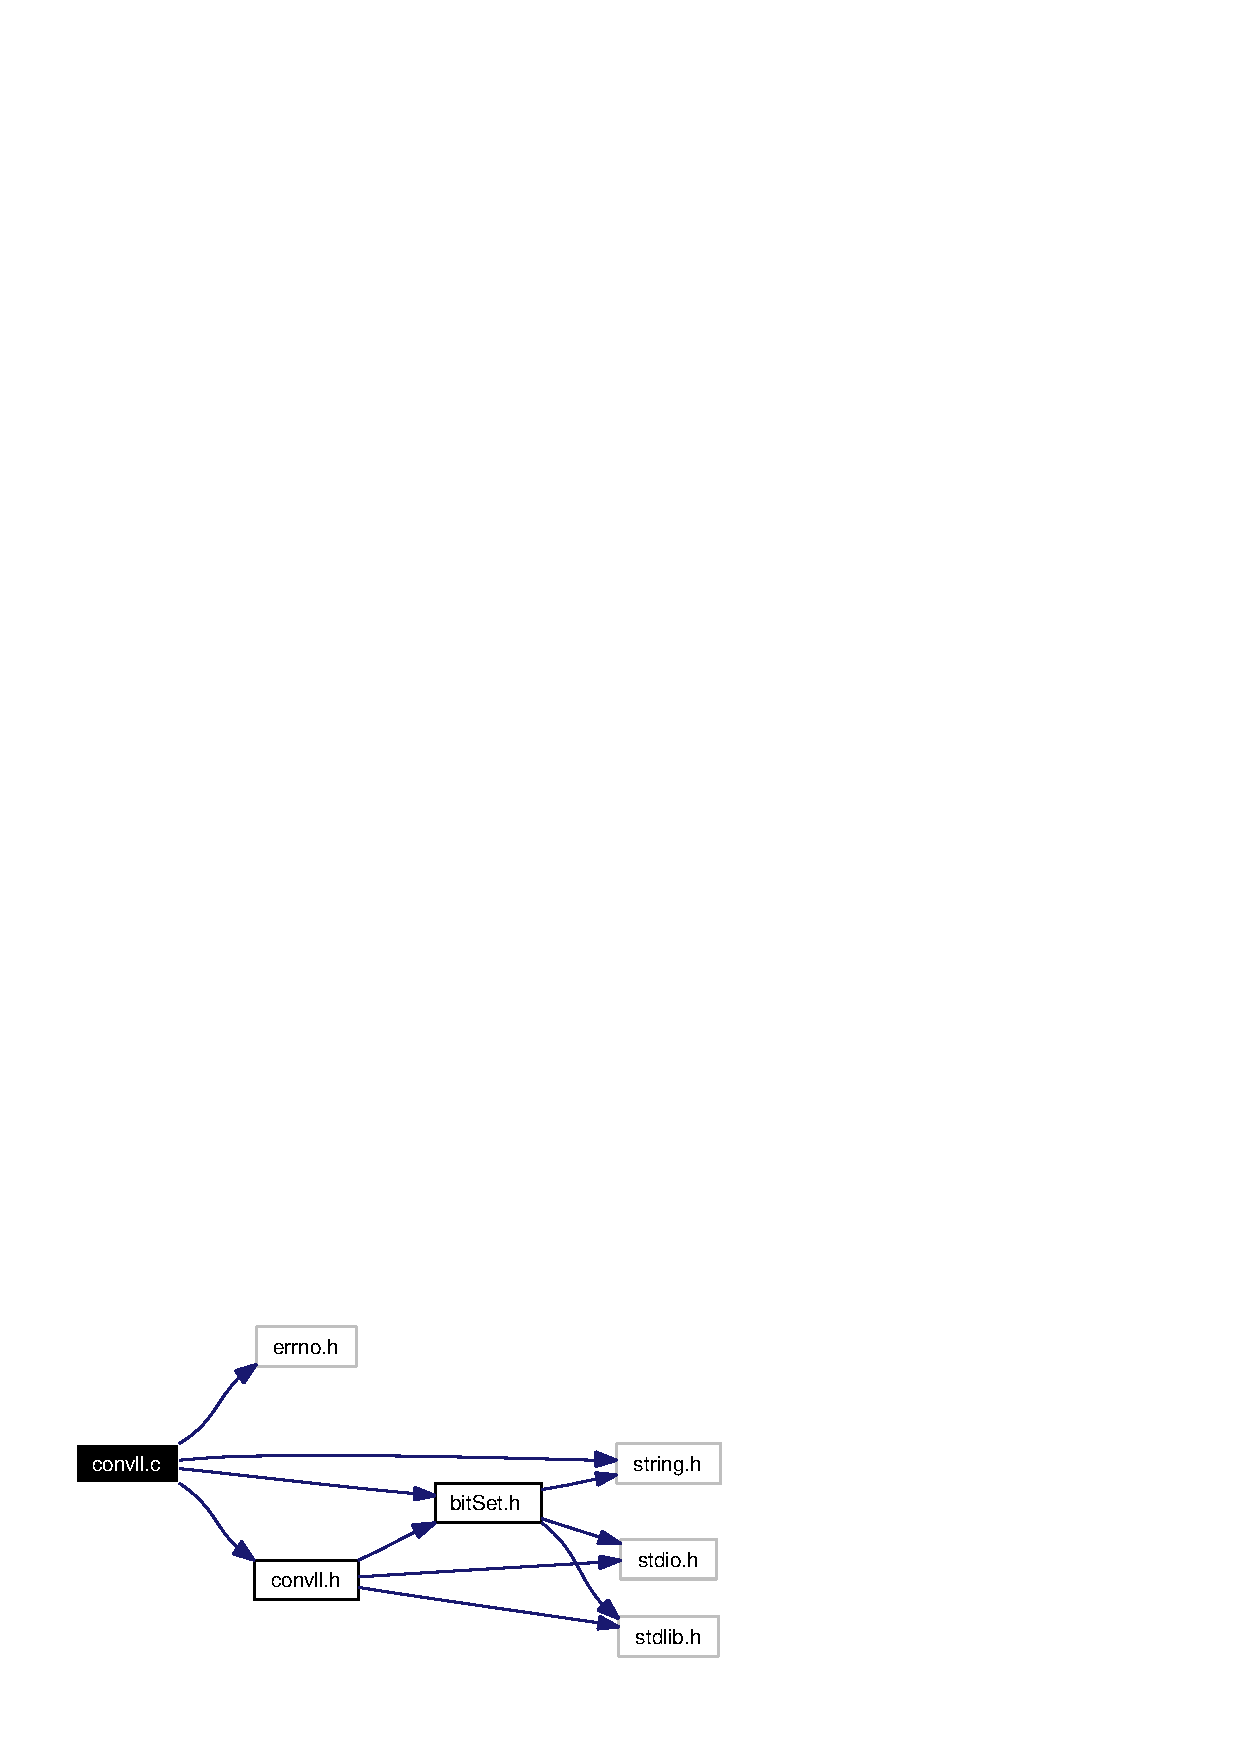
\includegraphics[width=173pt]{convll_8c__incl}
\end{center}
\end{figure}
\subsection*{Functions}
\begin{CompactItemize}
\item 
\hyperlink{structcnode}{cll\_\-t} $\ast$ \hyperlink{convll_8c_a1}{prune\-Cll} (\hyperlink{structcnode}{cll\_\-t} $\ast$head, int $\ast$index\-To\-Seq, int p)
\item 
\hyperlink{structcnode}{cll\_\-t} $\ast$ \hyperlink{convll_8c_a2}{push\-Cll} (\hyperlink{structcnode}{cll\_\-t} $\ast$head)
\item 
\hyperlink{structcnode}{cll\_\-t} $\ast$ \hyperlink{convll_8c_a3}{pop\-Cll} (\hyperlink{structcnode}{cll\_\-t} $\ast$head)
\item 
\hyperlink{structcnode}{cll\_\-t} $\ast$ \hyperlink{convll_8c_a4}{pop\-All\-Cll} (\hyperlink{structcnode}{cll\_\-t} $\ast$head)
\item 
int \hyperlink{convll_8c_a5}{print\-Cll} (\hyperlink{structcnode}{cll\_\-t} $\ast$head)
\item 
\hyperlink{structcnode}{cll\_\-t} $\ast$ \hyperlink{convll_8c_a6}{inithead\-Cll} (\hyperlink{structcnode}{cll\_\-t} $\ast$head, \hyperlink{structcSet__t}{c\-Set\_\-t} $\ast$newset)
\item 
\hyperlink{structcnode}{cll\_\-t} $\ast$ \hyperlink{convll_8c_a7}{pushc\-Set} (\hyperlink{structcnode}{cll\_\-t} $\ast$head, \hyperlink{structcSet__t}{c\-Set\_\-t} $\ast$newset)
\item 
\hyperlink{structcSet__t}{c\-Set\_\-t} $\ast$ \hyperlink{convll_8c_a8}{bit\-Set\-To\-CSet} (\hyperlink{structbitSet__t}{bit\-Set\_\-t} $\ast$clique)
\item 
int \hyperlink{convll_8c_a9}{check\-Cliquec\-Set} (\hyperlink{structcSet__t}{c\-Set\_\-t} $\ast$cliquec\-Set, int $\ast$index\-To\-Seq, int p)
\item 
\hyperlink{structcnode}{cll\_\-t} $\ast$ \hyperlink{convll_8c_a10}{push\-Clique} (\hyperlink{structbitSet__t}{bit\-Set\_\-t} $\ast$clique, \hyperlink{structcnode}{cll\_\-t} $\ast$head, int $\ast$index\-To\-Seq, int p)
\item 
\hyperlink{structmnode}{mll\_\-t} $\ast$ \hyperlink{convll_8c_a11}{push\-Mem\-Stack} (\hyperlink{structmnode}{mll\_\-t} $\ast$head, int clique\-Num)
\item 
\hyperlink{structmnode}{mll\_\-t} $\ast$ \hyperlink{convll_8c_a12}{pop\-Mem\-Stack} (\hyperlink{structmnode}{mll\_\-t} $\ast$head)
\item 
\hyperlink{structmnode}{mll\_\-t} $\ast$ \hyperlink{convll_8c_a13}{pop\-Whole\-Mem\-Stack} (\hyperlink{structmnode}{mll\_\-t} $\ast$head)
\item 
\hyperlink{structmnode}{mll\_\-t} $\ast$$\ast$ \hyperlink{convll_8c_a14}{add\-To\-Stacks} (\hyperlink{structcnode}{cll\_\-t} $\ast$node, \hyperlink{structmnode}{mll\_\-t} $\ast$$\ast$member\-Stacks)
\item 
\hyperlink{structmnode}{mll\_\-t} $\ast$$\ast$ \hyperlink{convll_8c_a15}{fill\-Member\-Stacks} (\hyperlink{structcnode}{cll\_\-t} $\ast$head, \hyperlink{structmnode}{mll\_\-t} $\ast$$\ast$member\-Stacks)
\item 
\hyperlink{structmnode}{mll\_\-t} $\ast$$\ast$ \hyperlink{convll_8c_a16}{empty\-Member\-Stacks} (\hyperlink{structmnode}{mll\_\-t} $\ast$$\ast$member\-Stacks, int size)
\item 
void \hyperlink{convll_8c_a17}{print\-Member\-Stacks} (\hyperlink{structmnode}{mll\_\-t} $\ast$$\ast$member\-Stacks, int size)
\item 
\hyperlink{structbitSet__t}{bit\-Set\_\-t} $\ast$ \hyperlink{convll_8c_a18}{set\-Stack\-True} (\hyperlink{structmnode}{mll\_\-t} $\ast$$\ast$mem\-List, int i, \hyperlink{structbitSet__t}{bit\-Set\_\-t} $\ast$queue)
\item 
\hyperlink{structbitSet__t}{bit\-Set\_\-t} $\ast$ \hyperlink{convll_8c_a19}{search\-Mems\-With\-List} (int $\ast$list, int listsize, \hyperlink{structmnode}{mll\_\-t} $\ast$$\ast$mem\-List, int num\-Offsets, \hyperlink{structbitSet__t}{bit\-Set\_\-t} $\ast$queue)
\item 
\hyperlink{structcnode}{cll\_\-t} $\ast$ \hyperlink{convll_8c_a20}{single\-Clique\-Conv} (\hyperlink{structcnode}{cll\_\-t} $\ast$head, int first\-Clique, \hyperlink{structcnode}{cll\_\-t} $\ast$$\ast$first\-Guess, int second\-Clique, \hyperlink{structcnode}{cll\_\-t} $\ast$$\ast$second\-Guess, \hyperlink{structcnode}{cll\_\-t} $\ast$next\-Phase, \hyperlink{structbitSet__t}{bit\-Set\_\-t} $\ast$print\-Status, int support)
\item 
\hyperlink{structmnode}{mll\_\-t} $\ast$ \hyperlink{convll_8c_a21}{merge\-Intersect} (\hyperlink{structcnode}{cll\_\-t} $\ast$first, \hyperlink{structcnode}{cll\_\-t} $\ast$second, \hyperlink{structmnode}{mll\_\-t} $\ast$intersection, \hyperlink{structbitSet__t}{bit\-Set\_\-t} $\ast$printstatus, int $\ast$new\-Support)
\item 
int \hyperlink{convll_8c_a22}{uniq\-Clique} (\hyperlink{structcSet__t}{c\-Set\_\-t} $\ast$cliquec\-Set, \hyperlink{structcnode}{cll\_\-t} $\ast$head)
\item 
\hyperlink{structcnode}{cll\_\-t} $\ast$ \hyperlink{convll_8c_a23}{swap\-Nodec\-Set} (\hyperlink{structcnode}{cll\_\-t} $\ast$head, int node, \hyperlink{structcSet__t}{c\-Set\_\-t} $\ast$new\-Clique)
\item 
\hyperlink{structcnode}{cll\_\-t} $\ast$ \hyperlink{convll_8c_a24}{remove\-Supers} (\hyperlink{structcnode}{cll\_\-t} $\ast$head, int node, \hyperlink{structcSet__t}{c\-Set\_\-t} $\ast$new\-Clique)
\item 
int \hyperlink{convll_8c_a25}{print\-CSet} (\hyperlink{structcSet__t}{c\-Set\_\-t} $\ast$node)
\item 
\hyperlink{structcnode}{cll\_\-t} $\ast$ \hyperlink{convll_8c_a26}{push\-Conv\-Clique} (\hyperlink{structmnode}{mll\_\-t} $\ast$clique, \hyperlink{structcnode}{cll\_\-t} $\ast$head)
\item 
\hyperlink{structcSet__t}{c\-Set\_\-t} $\ast$ \hyperlink{convll_8c_a27}{mll\-To\-CSet} (\hyperlink{structmnode}{mll\_\-t} $\ast$clique)
\item 
\hyperlink{structcnode}{cll\_\-t} $\ast$ \hyperlink{convll_8c_a28}{whole\-Clique\-Conv} (\hyperlink{structcnode}{cll\_\-t} $\ast$head, \hyperlink{structcnode}{cll\_\-t} $\ast$node, \hyperlink{structcnode}{cll\_\-t} $\ast$$\ast$first\-Guess, \hyperlink{structmnode}{mll\_\-t} $\ast$$\ast$mem\-List, int num\-Offsets, \hyperlink{structcnode}{cll\_\-t} $\ast$next\-Phase, \hyperlink{structbitSet__t}{bit\-Set\_\-t} $\ast$print\-Status, int support)
\item 
\hyperlink{structcnode}{cll\_\-t} $\ast$ \hyperlink{convll_8c_a29}{whole\-Round\-Conv} (\hyperlink{structcnode}{cll\_\-t} $\ast$$\ast$head, \hyperlink{structmnode}{mll\_\-t} $\ast$$\ast$mem\-List, int num\-Offsets, int support, int length, \hyperlink{structcnode}{cll\_\-t} $\ast$$\ast$all\-Cliques)
\item 
int \hyperlink{convll_8c_a30}{yank\-Cll} (\hyperlink{structcnode}{cll\_\-t} $\ast$$\ast$head, \hyperlink{structcnode}{cll\_\-t} $\ast$prev, \hyperlink{structcnode}{cll\_\-t} $\ast$$\ast$curr, \hyperlink{structcnode}{cll\_\-t} $\ast$$\ast$all\-Cliques, int length)
\item 
\hyperlink{structcnode}{cll\_\-t} $\ast$ \hyperlink{convll_8c_a31}{complete\-Conv} (\hyperlink{structcnode}{cll\_\-t} $\ast$$\ast$head, int support, int num\-Offsets, int min\-Length, int $\ast$index\-To\-Seq, int p)
\item 
int \hyperlink{convll_8c_a32}{print\-Cll\-Pattern} (\hyperlink{structcnode}{cll\_\-t} $\ast$node, int length)
\end{CompactItemize}
\subsection*{Variables}
\begin{CompactItemize}
\item 
int \hyperlink{convll_8c_a0}{cliquecounter} = 0
\end{CompactItemize}


\subsection*{Detailed Description}
This file defines a number of functions for handling link lists of motifs, or cliques. The functions defined in this file are called extensively during the convolution stage of the Gemoda algorithm for both the sequence based and real value based software.

Definition in file \hyperlink{convll_8c-source}{convll.c}.

\subsection*{Function Documentation}
\hypertarget{convll_8c_a14}{
\index{convll.c@{convll.c}!addToStacks@{addToStacks}}
\index{addToStacks@{addToStacks}!convll.c@{convll.c}}
\subsubsection[addToStacks]{\setlength{\rightskip}{0pt plus 5cm}\hyperlink{structmnode}{mll\_\-t}$\ast$$\ast$ add\-To\-Stacks (\hyperlink{structcnode}{cll\_\-t} $\ast$ {\em node}, \hyperlink{structmnode}{mll\_\-t} $\ast$$\ast$ {\em member\-Stacks})}}
\label{convll_8c_a14}


For one clique, it adds membership for that clique to all of its members' member stacks. Input: a specific clique in a clique linked list, an array of member stacks. Output: the array of updated member stacks.

Definition at line 482 of file convll.c.

References cnode::id, c\-Set\_\-t::members, push\-Mem\-Stack(), and cnode::set.

Referenced by fill\-Member\-Stacks().

\scriptsize\begin{verbatim}483 {
484   int i = 0;
485   int cliqueNum = 0;
486 
487   // Make sure that we don't reference NULL values
488   if (node->set != NULL)
489     {
490       // Go through each member of the clique's set
491       for (i = 0; i < node->set->size; i++)
492     {
493       // Get the member's number
494       cliqueNum = node->set->members[i];
495       // Go to that member's linked list and push
496       // on the number of the current clique
497       memberStacks[cliqueNum] =
498         pushMemStack (memberStacks[cliqueNum], node->id);
499     }
500     }
501   else
502     {
503       fprintf (stderr, "\nNULL set for clique! - addToStacks\n");
504       fflush (stderr);
505       exit (0);
506     }
507   return memberStacks;
508 }
\end{verbatim}
\normalsize 


\hypertarget{convll_8c_a8}{
\index{convll.c@{convll.c}!bitSetToCSet@{bitSetToCSet}}
\index{bitSetToCSet@{bitSetToCSet}!convll.c@{convll.c}}
\subsubsection[bitSetToCSet]{\setlength{\rightskip}{0pt plus 5cm}\hyperlink{structcSet__t}{c\-Set\_\-t}$\ast$ bit\-Set\-To\-CSet (\hyperlink{structbitSet__t}{bit\-Set\_\-t} $\ast$ {\em clique})}}
\label{convll_8c_a8}


Converts a \hyperlink{structbitSet__t}{bit\-Set\_\-t} to a \hyperlink{structcSet__t}{c\-Set\_\-t} for the purposes of pushing it onto a linked list of cliques. The \hyperlink{structbitSet__t}{bit\-Set\_\-t} data structure is used for massive comparisons during clique-finding but is unwieldy/inefficient when it is known that the structure is sparse. The \hyperlink{structcSet__t}{c\-Set\_\-t} allows for efficient comparison of sparse bit\-Set\_\-t's. Use this just before pushing a newly-discovered clique onto a clique linked list. Input: a new clique in the form of a \hyperlink{structbitSet__t}{bit\-Set\_\-t}. Output: the same clique in the form of a \hyperlink{structcSet__t}{c\-Set\_\-t}.

Definition at line 212 of file convll.c.

References count\-Set(), c\-Set\_\-t::members, next\-Bit\-Bit\-Set(), and c\-Set\_\-t::size.

Referenced by push\-Clique(), and whole\-Clique\-Conv().

\scriptsize\begin{verbatim}213 {
214   int cliqueSize = countSet (clique);
215   int i = 0, start = 0;
216   cSet_t *holder = (cSet_t *) malloc (sizeof (cSet_t));
217 
218   // Memory error checking
219   if (holder == NULL)
220     {
221       fprintf (stderr, "\nMemory Error - bitSetToCSet - [1]\n%s\n",
222            strerror (errno));
223       fflush (stderr);
224       exit (0);
225     }
226   // More memory checking
227   holder->members = (int *) malloc (cliqueSize * sizeof (int));
228   if (holder->members == NULL)
229     {
230       fprintf (stderr, "\nMemory Error - bitSetToCSet - [2]\n%s\n",
231            strerror (errno));
232       fflush (stderr);
233       exit (0);
234     }
235 
236   // For each member of the clique in the bitSet,
237   for (i = 0; i < cliqueSize; i++)
238     {
239       // Find the next one, add its location to the members array
240       holder->members[i] = nextBitBitSet (clique, start);
241       // (But check for errors... if we get to the end of the
242       // bitSet, then something is wrong)
243       if (holder->members[i] == -1)
244     {
245       fprintf (stderr, "\nClique error - not enough members\n");
246       fflush (stderr);
247       exit (0);
248     }
249       // Increment to move on in the nextBitBitSet search
250       start = holder->members[i] + 1;
251     }
252 
253   holder->size = cliqueSize;
254   return holder;
255 }
\end{verbatim}
\normalsize 


\hypertarget{convll_8c_a9}{
\index{convll.c@{convll.c}!checkCliquecSet@{checkCliquecSet}}
\index{checkCliquecSet@{checkCliquecSet}!convll.c@{convll.c}}
\subsubsection[checkCliquecSet]{\setlength{\rightskip}{0pt plus 5cm}int check\-Cliquec\-Set (\hyperlink{structcSet__t}{c\-Set\_\-t} $\ast$ {\em cliquec\-Set}, int $\ast$ {\em index\-To\-Seq}, int {\em p})}}
\label{convll_8c_a9}


Checks to enforce the -p flag (minimum number of unique input sequences in which the motif occurs). Input: a clique in the form of a \hyperlink{structcSet__t}{c\-Set\_\-t}, pointer to the index/sequence number data structure, the -p flag value. Output: An integer: 1 for success, 0 for failure.

Definition at line 266 of file convll.c.

References c\-Set\_\-t::members, and c\-Set\_\-t::size.

Referenced by push\-Clique().

\scriptsize\begin{verbatim}267 {
268   int *seqNums = NULL;
269   int thisSeq = 0, i = 0, j = 0;
270   seqNums = (int *) malloc (p * sizeof (int));
271 
272   if (seqNums == NULL)
273     {
274       fprintf (stderr, "Memory error - checkCliquecSet\n%s\n",
275            strerror (errno));
276       fflush (stderr);
277       exit (0);
278     }
279   // Initialize an array of integers of size p to sentinel values of -1
280   for (i = 0; i < p; i++)
281     {
282       seqNums[i] = -1;
283     }
284   j = 0;
285 
286   if (cliquecSet->size < 1)
287     {
288       fprintf (stderr, "\nClique of zero size! - checkCliquecSet\n");
289       fflush (stderr);
290       exit (0);
291     }
292   // Find the first sequence number.
293   seqNums[0] = indexToSeq[cliquecSet->members[0]];
294   // Iterate over the remaining size of the clique
295   for (i = 1; i < cliquecSet->size; i++)
296     {
297       // Find the next sequence number.
298       thisSeq = indexToSeq[cliquecSet->members[i]];
299       // The member list is in monotonic order, so we only need
300       // to compare the current member to the previous member to 
301       // find out if it comes from the same sequence.
302       // If it's not from the same sequence, increment the unique
303       // sequence counter (j), store the next sequence number
304       // in the array.
305       // Also check to see if we've already reached the p threshold,
306       // and if so, then bail out.
307       if (thisSeq != seqNums[j])
308     {
309       j++;
310       seqNums[j] = thisSeq;
311       if (j == p - 1)
312         {
313           break;
314         }
315     }
316     }
317 
318   // Now just see what the value of the last number in the array is;
319   // if it's the sentinel, then we didn't find instances in p 
320   // unique sequences.  If it's not the sentinel, then we've met
321   // the -p criterion.
322   if (seqNums[p - 1] == -1)
323     {
324       free (seqNums);
325       return (0);
326     }
327   else
328     {
329       free (seqNums);
330       return (1);
331     }
332 }
\end{verbatim}
\normalsize 


\hypertarget{convll_8c_a31}{
\index{convll.c@{convll.c}!completeConv@{completeConv}}
\index{completeConv@{completeConv}!convll.c@{convll.c}}
\subsubsection[completeConv]{\setlength{\rightskip}{0pt plus 5cm}\hyperlink{structcnode}{cll\_\-t}$\ast$ complete\-Conv (\hyperlink{structcnode}{cll\_\-t} $\ast$$\ast$ {\em head}, int {\em support}, int {\em num\-Offsets}, int {\em min\-Length}, int $\ast$ {\em index\-To\-Seq}, int {\em p})}}
\label{convll_8c_a31}


Performs complete convolution given the starting list of cliques. Input: a pointer to the head of the initial clique linked list, the minimum support criterion value, the number of offsets in the sequence set, the minimum length of motifs (which is the length of motifs in the initial clique linked list), the index/Sequence data structure, and the value of the -p flag to prune based on unique sequence occurrences. Output: a linked list of all maximal cliques based on the initial clique linked list.

Definition at line 1417 of file convll.c.

References empty\-Member\-Stacks(), fill\-Member\-Stacks(), pop\-All\-Cll(), prune\-Cll(), and whole\-Round\-Conv().

Referenced by convolve().

\scriptsize\begin{verbatim}1419 {
1420   int i = 0;
1421   mll_t **memList = NULL;
1422   cll_t *nextPhase = NULL;
1423   cll_t *allCliques = NULL;
1424   int length = minLength;
1425   memList = (mll_t **) malloc (numOffsets * sizeof (mll_t *));
1426   if (memList == NULL)
1427     {
1428       fprintf (stderr, "Memory error - completeConv\n%s\n", strerror (errno));
1429       fflush (stderr);
1430       exit (0);
1431     }
1432   // The number of offsets will never change, so this can be defined
1433   // now, though we will have to change what is in these arrays later.
1434   for (i = 0; i < numOffsets; i++)
1435     {
1436       memList[i] = NULL;
1437     }
1438 
1439   // NOTE: This assumes that the elemPats all meet the support criterion
1440 
1441   // So we'll do this as long as the head is non-null.. that means that 
1442   // the initial set of cliques must be non-null.  Those are then 
1443   // convolved and the linked list for the next round is set to head,
1444   // so this continues until the linked list for the "next round" at
1445   // the end of some round is null.
1446   while (*head != NULL)
1447     {
1448       // First we get the inverse information for this round: find
1449       // out which cliques each offset is a member of.
1450       memList = fillMemberStacks (*head, memList);
1451       // printf("numOffsets.bak = %d\n",numOffsets);
1452       // // Then we convolve a whole round.
1453       nextPhase =
1454     wholeRoundConv (head, memList, numOffsets, support, length,
1455             &allCliques);
1456       // Do some housekeeping.
1457       memList = emptyMemberStacks (memList, numOffsets);
1458       popAllCll (*head);
1459       // Enforce the -p flag for subsequent rounds.
1460       if (p > 1)
1461     {
1462       nextPhase = pruneCll (nextPhase, indexToSeq, p);
1463     }
1464       // And move on to the next round of convolution.
1465       *head = nextPhase;
1466       length++;
1467     }
1468 
1469   free (memList);
1470 
1471   return allCliques;
1472 }
\end{verbatim}
\normalsize 


\hypertarget{convll_8c_a16}{
\index{convll.c@{convll.c}!emptyMemberStacks@{emptyMemberStacks}}
\index{emptyMemberStacks@{emptyMemberStacks}!convll.c@{convll.c}}
\subsubsection[emptyMemberStacks]{\setlength{\rightskip}{0pt plus 5cm}\hyperlink{structmnode}{mll\_\-t}$\ast$$\ast$ empty\-Member\-Stacks (\hyperlink{structmnode}{mll\_\-t} $\ast$$\ast$ {\em member\-Stacks}, int {\em size})}}
\label{convll_8c_a16}


After we have performed a round of convolution, this \char`\"{}empties\char`\"{} the member stacks by popping all nodes off each member linked list. Input: array of member linked lists, the size of that array (total number of offsets). Output: the array of now-empty member linked lists.

Definition at line 538 of file convll.c.

References pop\-Whole\-Mem\-Stack().

Referenced by complete\-Conv().

\scriptsize\begin{verbatim}539 {
540   int i = 0;
541 
542   for (i = 0; i < size; i++)
543     {
544       memberStacks[i] = popWholeMemStack (memberStacks[i]);
545     }
546 
547   return memberStacks;
548 }
\end{verbatim}
\normalsize 


\hypertarget{convll_8c_a15}{
\index{convll.c@{convll.c}!fillMemberStacks@{fillMemberStacks}}
\index{fillMemberStacks@{fillMemberStacks}!convll.c@{convll.c}}
\subsubsection[fillMemberStacks]{\setlength{\rightskip}{0pt plus 5cm}\hyperlink{structmnode}{mll\_\-t}$\ast$$\ast$ fill\-Member\-Stacks (\hyperlink{structcnode}{cll\_\-t} $\ast$ {\em head}, \hyperlink{structmnode}{mll\_\-t} $\ast$$\ast$ {\em member\-Stacks})}}
\label{convll_8c_a15}


Fills the entire member\-Stacks data structure by calling add\-To\-Stacks for each clique in the clique linked list. Input: head of a clique linked list, array of member linked lists. Output: the array of updated member linked lists.

Definition at line 517 of file convll.c.

References add\-To\-Stacks(), and cnode::next.

Referenced by complete\-Conv().

\scriptsize\begin{verbatim}518 {
519   cll_t *curr = head;
520   // Just go down the linked list calling addToStacks
521   while (curr != NULL)
522     {
523       memberStacks = addToStacks (curr, memberStacks);
524       curr = curr->next;
525     }
526 
527   return memberStacks;
528 }
\end{verbatim}
\normalsize 


\hypertarget{convll_8c_a6}{
\index{convll.c@{convll.c}!initheadCll@{initheadCll}}
\index{initheadCll@{initheadCll}!convll.c@{convll.c}}
\subsubsection[initheadCll]{\setlength{\rightskip}{0pt plus 5cm}\hyperlink{structcnode}{cll\_\-t}$\ast$ inithead\-Cll (\hyperlink{structcnode}{cll\_\-t} $\ast$ {\em head}, \hyperlink{structcSet__t}{c\-Set\_\-t} $\ast$ {\em newset})}}
\label{convll_8c_a6}


Initializes the empty head of a linked list by adding a set to that head. Note: this is only called immediately after pushing onto a cll, because the push always creates a new empty head. This function should not be called by the user; see pushc\-Set. Input: head of a linked list, pointer to a \hyperlink{structcSet__t}{c\-Set\_\-t} list of clique members. Output: head of a linked list.

Definition at line 172 of file convll.c.

References cnode::set.

Referenced by pushc\-Set().

\scriptsize\begin{verbatim}173 {
174   // Check to make sure that the head is not already initialized.
175   if (head->set != NULL)
176     {
177       printf ("Stack head already initialized!");
178       exit (0);
179     }
180   // Make the head's set pointer point to the new set.
181   head->set = newset;
182   return head;
183 }
\end{verbatim}
\normalsize 


\hypertarget{convll_8c_a21}{
\index{convll.c@{convll.c}!mergeIntersect@{mergeIntersect}}
\index{mergeIntersect@{mergeIntersect}!convll.c@{convll.c}}
\subsubsection[mergeIntersect]{\setlength{\rightskip}{0pt plus 5cm}\hyperlink{structmnode}{mll\_\-t}$\ast$ merge\-Intersect (\hyperlink{structcnode}{cll\_\-t} $\ast$ {\em first}, \hyperlink{structcnode}{cll\_\-t} $\ast$ {\em second}, \hyperlink{structmnode}{mll\_\-t} $\ast$ {\em intersection}, \hyperlink{structbitSet__t}{bit\-Set\_\-t} $\ast$ {\em printstatus}, int $\ast$ {\em new\-Support})}}
\label{convll_8c_a21}


Convolves two cliques in a non-commutative manner. It finds which members of the first clique are immediately followed by a member in the second clique. Input: pointer to the location in the linked list of the first clique to be convolved, pointer to the location in the linked list of the second clique to be convolved, a member linked list used to store the intersection of the two cliques, the printstatus bit\-Set, and a pointer to an integer with the support of the clique formed by convolution. Output: a member linked list with the intersection of the two cliques, plus the side effect of that intersection's cardinality being stored in the integer pointed to by new\-Support.

Definition at line 759 of file convll.c.

References c\-Set\_\-t::members, push\-Mem\-Stack(), and cnode::set.

Referenced by single\-Clique\-Conv().

\scriptsize\begin{verbatim}761 {
762 
763   int i = 0, j = 0, status = 0;
764 
765   // Make sure we are still in-bounds, otherwise we bail out
766   // We'll refer to the offset currently being analyzed from the 
767   // first clique as the 'first offset' and the offset currently
768   // being analyzed from the second clique as the 'second offset'
769   while ((i < first->set->size) && (j < second->set->size))
770     {
771       // If the second offset is earlier than the first offset plus
772       // one, then we move on to the next possible second offset
773       if ((first->set->members[i] + 1) > second->set->members[j])
774     {
775       j++;
776     }
777       // If the second offset is later than the first offset plus
778       // one, then we move on the next possible first offset
779       else if ((first->set->members[i] + 1) < second->set->members[j])
780     {
781       i++;
782     }
783       // Otherwise, the second offset is equal to the first offset
784       // plus one, so we have an extendable node.  Push that on
785       // to the intersection stack, move both the first and second
786       // offsets to their respective next possible offsets, and 
787       // increment the support counter for the new clique (status)
788       else
789     {
790       intersection = pushMemStack (intersection, first->set->members[i]);
791       i++;
792       j++;
793       status++;
794     }
795     }
796 
797   // Send the value of the clique's new support out of this function
798   *newSupport = status;
799   return intersection;
800 }
\end{verbatim}
\normalsize 


\hypertarget{convll_8c_a27}{
\index{convll.c@{convll.c}!mllToCSet@{mllToCSet}}
\index{mllToCSet@{mllToCSet}!convll.c@{convll.c}}
\subsubsection[mllToCSet]{\setlength{\rightskip}{0pt plus 5cm}\hyperlink{structcSet__t}{c\-Set\_\-t}$\ast$ mll\-To\-CSet (\hyperlink{structmnode}{mll\_\-t} $\ast$ {\em clique})}}
\label{convll_8c_a27}


Turns a member linked list used to store the intersection of two cliques into something more useful: a \hyperlink{structcSet__t}{c\-Set\_\-t} structure. Input: a clique in mll\_\-t form. Output: a clique in \hyperlink{structcSet__t}{c\-Set\_\-t} form.

Definition at line 1145 of file convll.c.

References mnode::clique\-Membership, c\-Set\_\-t::members, mnode::next, and c\-Set\_\-t::size.

Referenced by push\-Conv\-Clique().

\scriptsize\begin{verbatim}1146 {
1147   int sizecount = 0, i = 0;
1148   cSet_t *cliqueCset = malloc (sizeof (cSet_t));
1149   mll_t *head = clique;
1150   if (cliqueCset == NULL)
1151     {
1152       fprintf (stderr, "Memory error - mllToCSet cSet\n%s\n",
1153            strerror (errno));
1154       fflush (stderr);
1155       exit (0);
1156     }
1157   // First count up how many members there are in the member linked list
1158   while (head != NULL)
1159     {
1160       sizecount++;
1161       head = head->next;
1162     }
1163 
1164   head = clique;
1165   cliqueCset->size = sizecount;
1166   cliqueCset->members = (int *) malloc (sizecount * sizeof (int));
1167 
1168   if (cliqueCset->members == NULL)
1169     {
1170       fprintf (stderr, "Memory error - mllTlCSet cliquemembers\n%s\n",
1171            strerror (errno));
1172       fflush (stderr);
1173       exit (0);
1174     }
1175   // In order to stay in the same format as with bitSet translation to
1176   // cSet, we ensure that the ids of the members are ascending with
1177   // ascending index number in the cSet.  This is accomplished by noting
1178   // that since the intersection members are pushed onto the stack,
1179   // a LIFO operation, that the first intersected nodes off the stack
1180   // will have the highest ids, so we will put them at the end of
1181   // the members array with the higher index values.
1182   for (i = sizecount - 1; i >= 0; i--)
1183     {
1184       cliqueCset->members[i] = head->cliqueMembership;
1185       head = head->next;
1186     }
1187 
1188   return cliqueCset;
1189 }
\end{verbatim}
\normalsize 


\hypertarget{convll_8c_a4}{
\index{convll.c@{convll.c}!popAllCll@{popAllCll}}
\index{popAllCll@{popAllCll}!convll.c@{convll.c}}
\subsubsection[popAllCll]{\setlength{\rightskip}{0pt plus 5cm}\hyperlink{structcnode}{cll\_\-t}$\ast$ pop\-All\-Cll (\hyperlink{structcnode}{cll\_\-t} $\ast$ {\em head})}}
\label{convll_8c_a4}


Shortcut function to pop all of the members of a linked list. Input: head of a linked list. Output: head of a now-empty linked list.

Definition at line 109 of file convll.c.

References pop\-Cll().

Referenced by complete\-Conv(), and main().

\scriptsize\begin{verbatim}110 {
111   while (head != NULL)
112     {
113       head = popCll (head);
114     }
115   return head;
116 }
\end{verbatim}
\normalsize 


\hypertarget{convll_8c_a3}{
\index{convll.c@{convll.c}!popCll@{popCll}}
\index{popCll@{popCll}!convll.c@{convll.c}}
\subsubsection[popCll]{\setlength{\rightskip}{0pt plus 5cm}\hyperlink{structcnode}{cll\_\-t}$\ast$ pop\-Cll (\hyperlink{structcnode}{cll\_\-t} $\ast$ {\em head})}}
\label{convll_8c_a3}


Removes the head of the clique linked list, returns the new head of the clique linked list, and frees the memory occupied by the old head. Input: head of a linked list. Output: head of a linked list.

Definition at line 66 of file convll.c.

References c\-Set\_\-t::members, cnode::next, and cnode::set.

Referenced by pop\-All\-Cll().

\scriptsize\begin{verbatim}67 {
68   // by default the new head is NULL...is important later
69   cll_t *newHead = NULL;
70   if (head == NULL)
71     {
72       fprintf (stderr, "\nCan't pop a null linked list\n");
73       fflush (stderr);
74       exit (0);
75     }
76   // unless this is the end of the linked list, set the new head
77   // to the next member of the list.  Otherwise, since by default the
78   // new head is NULL, it will properly return an empty list
79   if (head->next != NULL)
80     {
81       newHead = head->next;
82     }
83   // Check to see if there is a set.  If there is, and there are members,
84   // then first free the members.  And if there is a set, then free it.
85   if (head->set != NULL)
86     {
87       if (head->set->members != NULL)
88     {
89       free (head->set->members);
90       head->set->members = NULL;
91     }
92       free (head->set);
93       head->set = NULL;
94     }
95   // Both the members and set have been freed, so now can free the cll_t
96   // without leaking anything.
97 
98   free (head);
99   head = NULL;
100   return newHead;
101 }
\end{verbatim}
\normalsize 


\hypertarget{convll_8c_a12}{
\index{convll.c@{convll.c}!popMemStack@{popMemStack}}
\index{popMemStack@{popMemStack}!convll.c@{convll.c}}
\subsubsection[popMemStack]{\setlength{\rightskip}{0pt plus 5cm}\hyperlink{structmnode}{mll\_\-t}$\ast$ pop\-Mem\-Stack (\hyperlink{structmnode}{mll\_\-t} $\ast$ {\em head})}}
\label{convll_8c_a12}


Pops the head off of a single member linked list. Input: head of a member linked list. Output: the new head of a member linked list after popping one item.

Definition at line 440 of file convll.c.

References mnode::next.

Referenced by pop\-Whole\-Mem\-Stack().

\scriptsize\begin{verbatim}441 {
442   // by default the new head is NULL...is important later
443   mll_t *newHead = NULL;
444   if (head == NULL)
445     {
446       fprintf (stderr, "\nCan't pop a null linked list - popMemStack\n");
447       fflush (stderr);
448       exit (0);
449     }
450   if (head->next != NULL)
451     {
452       newHead = head->next;
453     }
454   free (head);
455   head = NULL;
456   return newHead;
457 }
\end{verbatim}
\normalsize 


\hypertarget{convll_8c_a13}{
\index{convll.c@{convll.c}!popWholeMemStack@{popWholeMemStack}}
\index{popWholeMemStack@{popWholeMemStack}!convll.c@{convll.c}}
\subsubsection[popWholeMemStack]{\setlength{\rightskip}{0pt plus 5cm}\hyperlink{structmnode}{mll\_\-t}$\ast$ pop\-Whole\-Mem\-Stack (\hyperlink{structmnode}{mll\_\-t} $\ast$ {\em head})}}
\label{convll_8c_a13}


Pops all items off of a member linked list. Input: head of a member linked list. Output: empty head of a member linked list.

Definition at line 465 of file convll.c.

References pop\-Mem\-Stack().

Referenced by empty\-Member\-Stacks(), and single\-Clique\-Conv().

\scriptsize\begin{verbatim}466 {
467   while (head != NULL)
468     {
469       head = popMemStack (head);
470     }
471   return head;
472 }
\end{verbatim}
\normalsize 


\hypertarget{convll_8c_a5}{
\index{convll.c@{convll.c}!printCll@{printCll}}
\index{printCll@{printCll}!convll.c@{convll.c}}
\subsubsection[printCll]{\setlength{\rightskip}{0pt plus 5cm}int print\-Cll (\hyperlink{structcnode}{cll\_\-t} $\ast$ {\em head})}}
\label{convll_8c_a5}


Prints the members (cliques) of a linked list in the format: {\em id\/} = unique id number of clique within linked list; {\em Length\/} = number of members of clique, if available; {\em Size\/} = length of each member of clique; {\em Members\/} = newline-separated list of members of the clique. Input: head of a linked list. Output: Gives text output, returns (meaningless) exit value.

Definition at line 128 of file convll.c.

References cnode::id, cnode::length, c\-Set\_\-t::members, cnode::next, cnode::set, and c\-Set\_\-t::size.

\scriptsize\begin{verbatim}129 {
130   int i = 0;
131   cll_t *curr = head;
132   while (curr != NULL)
133     {
134       printf ("id = %d\n", curr->id);
135       // Make sure the clique is nonzero in size before attempting
136       // to print it
137       if ((curr->set != NULL) && (curr->set->size > 0))
138     {
139       if (curr->length >= 0)
140         {
141           printf ("Length = %d\n", curr->length);
142         }
143       printf ("Size = %d\n", curr->set->size);
144       printf ("Members = \n");
145       for (i = 0; i < curr->set->size; i++)
146         {
147           printf ("\t%d\n", curr->set->members[i]);
148         }
149       printf ("***********************************************\n");
150     }
151       else
152     {
153       fprintf (stderr, "\nClique has no members! -- printCll\n");
154       fflush (stderr);
155       exit (0);
156     }
157       curr = curr->next;
158     }
159   return EXIT_SUCCESS;
160 }
\end{verbatim}
\normalsize 


\hypertarget{convll_8c_a32}{
\index{convll.c@{convll.c}!printCllPattern@{printCllPattern}}
\index{printCllPattern@{printCllPattern}!convll.c@{convll.c}}
\subsubsection[printCllPattern]{\setlength{\rightskip}{0pt plus 5cm}int print\-Cll\-Pattern (\hyperlink{structcnode}{cll\_\-t} $\ast$ {\em node}, int {\em length})}}
\label{convll_8c_a32}


Prints out the contents of a clique linked list node in this format: {\em support\/} = number of motif occurrences ({\em id\/} = some id number); {\em members\/} = newline-separated list of offsets. Input: a specific node to be output, the length of the motif inside it. Output: text per above, and an integer success value.

Definition at line 1482 of file convll.c.

References cnode::id, c\-Set\_\-t::members, cnode::set, and c\-Set\_\-t::size.

\scriptsize\begin{verbatim}1483 {
1484   int i = 0;
1485 
1486   printf ("\nSupport = %d\t(id = %d)\n", node->set->size, node->id);
1487   printf ("Members = \n");
1488   for (i = 0; i < node->set->size; i++)
1489     {
1490       printf ("\t%d\n", node->set->members[i]);
1491     }
1492   return 1;
1493 }
\end{verbatim}
\normalsize 


\hypertarget{convll_8c_a25}{
\index{convll.c@{convll.c}!printCSet@{printCSet}}
\index{printCSet@{printCSet}!convll.c@{convll.c}}
\subsubsection[printCSet]{\setlength{\rightskip}{0pt plus 5cm}int print\-CSet (\hyperlink{structcSet__t}{c\-Set\_\-t} $\ast$ {\em node})}}
\label{convll_8c_a25}


Prints out the contents of a \hyperlink{structcSet__t}{c\-Set\_\-t} in the following format: {\em support\/} = number of nodes in clique; {\em members\/} = newline-separated list of nodes in clique. Input: a clique in the form of a \hyperlink{structcSet__t}{c\-Set\_\-t} object. Output: in text, the contents of the \hyperlink{structcSet__t}{c\-Set\_\-t} object. An integer is returned as well, with 1 indicating success.

Definition at line 1068 of file convll.c.

References c\-Set\_\-t::members, and c\-Set\_\-t::size.

\scriptsize\begin{verbatim}1069 {
1070   int i = 0;
1071   if (node->size == 0)
1072     {
1073       fprintf (stderr, "cSet has no members! - printCSet\n");
1074       fflush (stderr);
1075       exit (0);
1076     }
1077   else
1078     {
1079       printf ("\nSupport = %d\n", node->size);
1080       printf ("Members = \n");
1081       for (i = 0; i < node->size; i++)
1082     {
1083       printf ("\t%d\n", node->members[i]);
1084     }
1085       return 1;
1086     }
1087 }
\end{verbatim}
\normalsize 


\hypertarget{convll_8c_a17}{
\index{convll.c@{convll.c}!printMemberStacks@{printMemberStacks}}
\index{printMemberStacks@{printMemberStacks}!convll.c@{convll.c}}
\subsubsection[printMemberStacks]{\setlength{\rightskip}{0pt plus 5cm}void print\-Member\-Stacks (\hyperlink{structmnode}{mll\_\-t} $\ast$$\ast$ {\em member\-Stacks}, int {\em size})}}
\label{convll_8c_a17}


Prints the contents of the member stacks. Input: array of member linked lists, size of that array (total number of offsets). Output: only text output/no return value.

Definition at line 557 of file convll.c.

References mnode::clique\-Membership, and mnode::next.

\scriptsize\begin{verbatim}558 {
559   int i = 0;
560   mll_t *curr = NULL;
561 
562   for (i = 0; i < size; i++)
563     {
564       curr = memberStacks[i];
565       printf ("Offset %d: ", i);
566       while (curr != NULL)
567     {
568       printf ("%d,", curr->cliqueMembership);
569       curr = curr->next;
570     }
571       printf ("\n");
572     }
573 }
\end{verbatim}
\normalsize 


\hypertarget{convll_8c_a1}{
\index{convll.c@{convll.c}!pruneCll@{pruneCll}}
\index{pruneCll@{pruneCll}!convll.c@{convll.c}}
\subsubsection[pruneCll]{\setlength{\rightskip}{0pt plus 5cm}\hyperlink{structcnode}{cll\_\-t}$\ast$ prune\-Cll (\hyperlink{structcnode}{cll\_\-t} $\ast$ {\em head}, int $\ast$ {\em index\-To\-Seq}, int {\em p})}}
\label{convll_8c_a1}


Prunes a motif linked list of all motifs without support in at least

unique source sequences. Input: head of a motif linked list, pointer to a structure that dereferences offset indices to sequence numbers, minimum number of unique source sequences in which a motif must occur. Output: head of a (potentially altered) motif linked list.

Definition at line 514 of file new\-Conv.c.

References c\-Set\_\-t::members, cnode::next, cnode::set, and c\-Set\_\-t::size.

Referenced by complete\-Conv(), and convolve().

\scriptsize\begin{verbatim}515 {
516   int i = 0, j = 0, thisSeq = 0;
517   int *seqNums = NULL;
518   cll_t * curr = head;
519   cll_t * prev = NULL;
520   cll_t * storage = NULL;
521   
522     // We'll do this similar to the pruneBitGraph function... we will
523     // keep track of which source sequence each motif occurrence was in.
524     // Again, since the occurrences are listed monotonically, we only
525     // need to compare the last non-sentinel index to the current
526     // sequence number.
527     seqNums = (int *) malloc (p * sizeof (int));
528   if (seqNums == NULL)
529     {
530       fprintf (stderr, "Memory error - pruneCll\n%s\n", strerror (errno));
531       fflush (stderr);
532       exit (0);
533     }
534   while (curr != NULL)
535     {
536       
537     // First make sure the set size is at least p.
538     // This is redundant, but extremely simple and not expensive,
539     // so we'll leave it in just as a check.
540     if (curr->set->size < p)
541     {
542       if (prev != NULL)
543         {
544           prev->next = curr->next;
545         }
546       else
547         {
548           head = curr->next;
549         }
550       storage = curr->next;
551       free (curr->set->members);
552       free (curr->set);
553       free (curr);
554       curr = storage;
555       continue;
556     }
557       for (i = 0; i < p; i++)
558     {
559       seqNums[i] = -1;
560     }
561       j = 0;
562       seqNums[0] = indexToSeq[curr->set->members[0]];
563       
564     // Note, we've checked to make sure size > p, and we know
565     // p must be 2 or greater, so we can start at 1 without
566     // worrying about segfaulting
567     for (i = 1; i < curr->set->size; i++)
568     {
569       thisSeq = indexToSeq[curr->set->members[i]];
570       if (thisSeq != seqNums[j])
571         {
572           j++;
573           seqNums[j] = thisSeq;
574           if (j == p - 1)
575         {
576           break;
577         }
578         }
579     }
580       
581     // Same story as before... if the last number is -1,
582     // then we didn't have enough to fill up the <p> different
583     // slots, so this doesn't meet our criterion.
584     if (seqNums[p - 1] == -1)
585     {
586       if (prev != NULL)
587         {
588           prev->next = curr->next;
589         }
590       else
591         {
592           head = curr->next;
593         }
594       storage = curr->next;
595       free (curr->set->members);
596       free (curr->set);
597       free (curr);
598       curr = storage;
599     }
600       else
601     {
602       prev = curr;
603       curr = curr->next;
604     }
605     }
606   free (seqNums);
607   return (head);
608 }
\end{verbatim}
\normalsize 


\hypertarget{convll_8c_a10}{
\index{convll.c@{convll.c}!pushClique@{pushClique}}
\index{pushClique@{pushClique}!convll.c@{convll.c}}
\subsubsection[pushClique]{\setlength{\rightskip}{0pt plus 5cm}\hyperlink{structcnode}{cll\_\-t}$\ast$ push\-Clique (\hyperlink{structbitSet__t}{bit\-Set\_\-t} $\ast$ {\em clique}, \hyperlink{structcnode}{cll\_\-t} $\ast$ {\em head}, int $\ast$ {\em index\-To\-Seq}, int {\em p})}}
\label{convll_8c_a10}


Pushes a bit\-Set onto a clique linked list, performing all necessary manipulations in order to do so. Input: new clique in the form of a \hyperlink{structbitSet__t}{bit\-Set\_\-t}, head of a linked list, pointer to the index/sequence number data structure, integer value of the -p flag. Output: head of an updated clique linked list.

Definition at line 345 of file convll.c.

References bit\-Set\-To\-CSet(), check\-Cliquec\-Set(), cliquecounter, and pushc\-Set().

Referenced by find\-Cliques(), and single\-Linkage().

\scriptsize\begin{verbatim}346 {
347   cSet_t *cliquecSet = NULL;
348 
349   // Change the bitSet_t to a cSet_t
350   cliquecSet = bitSetToCSet (clique);
351   // If the -p flag has been assigned a value, then check the clique
352   // and only proceed if that criterion is met.  Otherwise, free the
353   // memory that we had allocated up to this point.
354   if (p > 1)
355     {
356       if (checkCliquecSet (cliquecSet, indexToSeq, p))
357     {
358       cliquecounter++;
359       /*
360          printf("%d\n",cliquecounter);
361        */
362       /*
363          fflush(stdout);
364        */
365       head = pushcSet (head, cliquecSet);
366     }
367       else
368     {
369       free (cliquecSet->members);
370       free (cliquecSet);
371     }
372       // If the -p flag wasn't set, then just push the cSet onto the linked
373       // list.
374     }
375   else
376     {
377       cliquecounter++;
378       /*
379          printf("%d\n",cliquecounter);
380        */
381       /*
382          fflush(stdout);
383        */
384       head = pushcSet (head, cliquecSet);
385     }
386   return head;
387 }
\end{verbatim}
\normalsize 


\hypertarget{convll_8c_a2}{
\index{convll.c@{convll.c}!pushCll@{pushCll}}
\index{pushCll@{pushCll}!convll.c@{convll.c}}
\subsubsection[pushCll]{\setlength{\rightskip}{0pt plus 5cm}\hyperlink{structcnode}{cll\_\-t}$\ast$ push\-Cll (\hyperlink{structcnode}{cll\_\-t} $\ast$ {\em head})}}
\label{convll_8c_a2}


Pushes a new, empty head onto a linked list of cliques. Note: this should always be followed by a call to inithead\-Cll, as the head pushed on here is empty and will be meaningless without any members. This function should NOT be used by the user; see pushc\-Set. Input: head of a linked list. Output: head of a linked list.

Definition at line 28 of file convll.c.

References cnode::id, cnode::length, cnode::next, cnode::set, and cnode::stat.

Referenced by pushc\-Set().

\scriptsize\begin{verbatim}29 {
30   // Make a pointer, verify memory
31   cll_t *a = NULL;
32   a = (cll_t *) malloc (sizeof (cll_t));
33   if (a == NULL)
34     {
35       fprintf (stderr, "\nMemory Error - pushCll\n%s\n", strerror (errno));
36       fflush (stderr);
37       exit (0);
38     }
39   // Initialize id (sequential) and pointer to next item, but not
40   // the cSet with the clique members
41   if (head == NULL)
42     {
43       a->id = 0;
44       a->next = NULL;
45     }
46   else
47     {
48       a->next = head;
49       a->id = head->id + 1;
50     }
51   a->set = NULL;
52   a->length = -1;
53   a->stat = -1;
54   return a;
55 }
\end{verbatim}
\normalsize 


\hypertarget{convll_8c_a26}{
\index{convll.c@{convll.c}!pushConvClique@{pushConvClique}}
\index{pushConvClique@{pushConvClique}!convll.c@{convll.c}}
\subsubsection[pushConvClique]{\setlength{\rightskip}{0pt plus 5cm}\hyperlink{structcnode}{cll\_\-t}$\ast$ push\-Conv\-Clique (\hyperlink{structmnode}{mll\_\-t} $\ast$ {\em clique}, \hyperlink{structcnode}{cll\_\-t} $\ast$ {\em head})}}
\label{convll_8c_a26}


Pushes a freshly-convolved clique, currently in mll\_\-t form, onto the clique linked list for the next level. Also checks to make sure that the convolved clique is unique, and if it isn't, it takes appropriate action. Input: a convolved clique in mll\_\-t form, the head of a clique linked list for the next level. Output: (potentially new) head of the clique linked list for the next level.

Definition at line 1099 of file convll.c.

References c\-Set\_\-t::members, mll\-To\-CSet(), pushc\-Set(), remove\-Supers(), swap\-Nodec\-Set(), and uniq\-Clique().

Referenced by single\-Clique\-Conv().

\scriptsize\begin{verbatim}1100 {
1101   int status = 0;
1102   cSet_t *cliquecSet = NULL;
1103 
1104   // First change the clique to something we can used more easily
1105   cliquecSet = mllToCSet (clique);
1106   // Then check to make sure it's unique by finding out its status
1107   status = uniqClique (cliquecSet, head);
1108 
1109   // printf("Candidate:\n");
1110   // printCSet(cliquecSet);
1111 
1112   // If we get -2, then this clique is a subset, so just free 
1113   // the cSet we just made and move on.
1114   if (status == -2)
1115     {
1116       free (cliquecSet->members);
1117       free (cliquecSet);
1118       cliquecSet = NULL;
1119     }
1120   // If we get -1, then this is a unique clique, so push it on.
1121   else if (status == -1)
1122     {
1123       head = pushcSet (head, cliquecSet);
1124     }
1125   // Otherwise, this clique is a superset, so we'll first remove
1126   // all of the other cliques of which this is a superset.  Then
1127   // we'll swap out the first clique of which this is a superset
1128   // with this current clique.  The clique being removed is free'd 
1129   // within the swapNode function.
1130   else
1131     {
1132       head = removeSupers (head, status, cliquecSet);
1133       head = swapNodecSet (head, status, cliquecSet);
1134     }
1135   return head;
1136 }
\end{verbatim}
\normalsize 


\hypertarget{convll_8c_a7}{
\index{convll.c@{convll.c}!pushcSet@{pushcSet}}
\index{pushcSet@{pushcSet}!convll.c@{convll.c}}
\subsubsection[pushcSet]{\setlength{\rightskip}{0pt plus 5cm}\hyperlink{structcnode}{cll\_\-t}$\ast$ pushc\-Set (\hyperlink{structcnode}{cll\_\-t} $\ast$ {\em head}, \hyperlink{structcSet__t}{c\-Set\_\-t} $\ast$ {\em newset})}}
\label{convll_8c_a7}


Function that pushes the contents of a c\-Set (set of members of a clique) onto a linked list of cliques. Input: head of a linked list, new clique in the form of a \hyperlink{structcSet__t}{c\-Set\_\-t}. Output: head of a linked list.

Definition at line 192 of file convll.c.

References inithead\-Cll(), and push\-Cll().

Referenced by push\-Clique(), and push\-Conv\-Clique().

\scriptsize\begin{verbatim}193 {
194   head = pushCll (head);
195   head = initheadCll (head, newset);
196   return head;
197 }
\end{verbatim}
\normalsize 


\hypertarget{convll_8c_a11}{
\index{convll.c@{convll.c}!pushMemStack@{pushMemStack}}
\index{pushMemStack@{pushMemStack}!convll.c@{convll.c}}
\subsubsection[pushMemStack]{\setlength{\rightskip}{0pt plus 5cm}\hyperlink{structmnode}{mll\_\-t}$\ast$ push\-Mem\-Stack (\hyperlink{structmnode}{mll\_\-t} $\ast$ {\em head}, int {\em clique\-Num})}}
\label{convll_8c_a11}


This begins code for the member linked lists. A single one of these linked lists functions somewhat similarly to the clique linked lists, though with less information stored. Functionally, an array of member linked lists is used to access the \char`\"{}inverse\char`\"{} of what is contained in the clique linked lists. That is, we would like to be able to look up the cliques that a given node is a member of, so we have an array of member linked lists of size equal to the number of nodes.

This function pushes a single clique membership onto a node's member stack. Input: the head of a single member linked list, a clique number to be added. Output: the head of a single member linked list.

Definition at line 404 of file convll.c.

References mnode::clique\-Membership, and mnode::next.

Referenced by add\-To\-Stacks(), and merge\-Intersect().

\scriptsize\begin{verbatim}405 {
406   mll_t *a = NULL;
407   a = (mll_t *) malloc (sizeof (mll_t));
408   // Memory error checking
409   if (a == NULL)
410     {
411       fprintf (stderr, "\nMemory Error - pushMemStack: %s\n",
412            strerror (errno));
413       fflush (stderr);
414       exit (0);
415     }
416   if (head == NULL)
417     {
418       a->next = NULL;
419     }
420   else
421     {
422       a->next = head;
423     }
424   // Store the number of the clique of which the node is a member.
425   // Note that we assume no duplication, which is guaranteed
426   // by our method of filling the member stacks, which is quite simple:
427   // go through all members of a clique (which have no duplicates
428   // because they are constructed from merge-intersections or from
429   // bitSet_t's) and add that clique to each node's membership list.
430   a->cliqueMembership = cliqueNum;
431   return a;
432 }
\end{verbatim}
\normalsize 


\hypertarget{convll_8c_a24}{
\index{convll.c@{convll.c}!removeSupers@{removeSupers}}
\index{removeSupers@{removeSupers}!convll.c@{convll.c}}
\subsubsection[removeSupers]{\setlength{\rightskip}{0pt plus 5cm}\hyperlink{structcnode}{cll\_\-t}$\ast$ remove\-Supers (\hyperlink{structcnode}{cll\_\-t} $\ast$ {\em head}, int {\em node}, \hyperlink{structcSet__t}{c\-Set\_\-t} $\ast$ {\em new\-Clique})}}
\label{convll_8c_a24}


This function finds all cliques in a linked list of which the proposed clique is a superset. It starts looking AFTER the first clique which has already been found to be a subset. In some senses, it is just a continuation of the uniqclique function in order to take advantage of the fact that though a proposed clique can only be a subset of one existing next-level clique, it can be a superset of many existing next- level cliques. Input: head of a clique linked list, the id of the first node found to be a subset of the proposed clique, and the proposed clique (in \hyperlink{structcSet__t}{c\-Set\_\-t} form). Output: the head of the clique linked list with all but the first subset (which was passed as an argument) removed. This function is now ready for swap\-Node to be called.

Definition at line 952 of file convll.c.

References cnode::id, c\-Set\_\-t::members, cnode::next, cnode::set, and c\-Set\_\-t::size.

Referenced by push\-Conv\-Clique().

\scriptsize\begin{verbatim}953 {
954   int foundStatus = 0;
955   cll_t *curr = head;
956   cll_t *prev = NULL;
957   int i = 0, j = 0, breakFlag = 0;
958 
959   while (curr != NULL)
960     {
961       if (curr->id == node)
962     {
963       foundStatus = 1;
964       break;
965     }
966       curr = curr->next;
967     }
968 
969   if (foundStatus == 0)
970     {
971       fprintf (stderr, "\nFirst clique not found! (removeSupers)\n");
972       fflush (stderr);
973       exit (0);
974     }
975   // Now this is trickier, to remove nodes from the middle of a linked
976   // list; this means that we need to remember which node we were just
977   // at so that we can connect it to the node after the one we are 
978   // about to delete.
979   prev = curr;
980   curr = curr->next;
981 
982   // This code is similar to that in uniqClique.
983   // Descend through all members of the next level's linked list.
984   while (curr != NULL)
985     {
986       i = 0;
987       j = 0;
988       breakFlag = 0;
989       // The proposed convolved clique will be referred to as the
990       // 'first' clique, and the current clique being analyzed
991       // in the next level is the 'second' clique.
992       // Continue if we have more members in both cliques.  We will
993       // have already broken out if it is not possible for this
994       // second clique to be a subset of the first.
995       while ((i < newClique->size) && (j < curr->set->size))
996     {
997       // If the current member of the first clique is
998       // less than the current member of the second clique
999       // then it is still possible that the first is a 
1000       // superset of the second, so move on to the next
1001       // member.
1002       if (newClique->members[i] < curr->set->members[j])
1003         {
1004           i++;
1005         }
1006       // If the current member of the first clique is greater
1007       // than the current member of the second clique, then
1008       // the proposed second clique cannot be a subset since
1009       // its members are all in ascending order.  We also
1010       // know that since the first clique already has
1011       // a subset in this linked list, the current node
1012       // cannot possibly be a superset of the proposed
1013       // clique, so we can just disregard that.  Thus,
1014       // we make a flag signifying this and break out.
1015       else if (newClique->members[i] > curr->set->members[j])
1016         {
1017           breakFlag = 1;
1018           break;
1019         }
1020       else
1021         {
1022           i++;
1023           j++;
1024         }
1025     }
1026       // If the breakflag is 1, then we know
1027       // that there is a member of the second clique not in the
1028       // first, and so the second is not a subset.  If the breakflag
1029       // is 0 but j is less than the second clique's size, then 
1030       // we must have broken because we ran out of members in the
1031       // first clique... thus, there is a member of the second 
1032       // clique not in the first.  Thus, only if the breakflag is
1033       // 0 and j is equal to the size of the second clique do we
1034       // know that every member of the second clique is in the first
1035       // and that the second clique can thus be removed.
1036       if ((breakFlag == 0) && (j == curr->set->size))
1037     {
1038       // Make the previous clique point to the next one
1039       // instead of the current one.
1040       prev->next = curr->next;
1041       // Free all of the memory used by the current clique.
1042       free (curr->set->members);
1043       free (curr->set);
1044       free (curr);
1045       curr = prev->next;
1046     }
1047       else
1048     {
1049       // Otherwise, the current second clique is not a 
1050       // subset of the first, and we advance the prev and
1051       // curr pointers.
1052       prev = curr;
1053       curr = curr->next;
1054     }
1055     }
1056   return head;
1057 }
\end{verbatim}
\normalsize 


\hypertarget{convll_8c_a19}{
\index{convll.c@{convll.c}!searchMemsWithList@{searchMemsWithList}}
\index{searchMemsWithList@{searchMemsWithList}!convll.c@{convll.c}}
\subsubsection[searchMemsWithList]{\setlength{\rightskip}{0pt plus 5cm}\hyperlink{structbitSet__t}{bit\-Set\_\-t}$\ast$ search\-Mems\-With\-List (int $\ast$ {\em list}, int {\em listsize}, \hyperlink{structmnode}{mll\_\-t} $\ast$$\ast$ {\em mem\-List}, int {\em num\-Offsets}, \hyperlink{structbitSet__t}{bit\-Set\_\-t} $\ast$ {\em queue})}}
\label{convll_8c_a19}


Creates one large queue by calling \char`\"{}set\-Stack\-True\char`\"{} for each member of a list of offsets. This then creates the union of clique membership for all offsets in the list being searched. Input: an array of offset numbers, the length of that array, an array of member linked lists, the length of that array (the total number of offsets), and a \hyperlink{structbitSet__t}{bit\-Set\_\-t} to store the union/queue. Output: the union/queue in a \hyperlink{structbitSet__t}{bit\-Set\_\-t} structure.

Definition at line 611 of file convll.c.

References empty\-Set(), and set\-Stack\-True().

Referenced by whole\-Clique\-Conv().

\scriptsize\begin{verbatim}613 {
614   int i = 0;
615   emptySet (queue);
616 
617   // Go through each offset in the list
618   for (i = 0; i < listsize; i++)
619     {
620       // Check to make sure that's a valid offset number, and if so
621       // then set its stack true in the queue.
622       if (list[i] + 1 < numOffsets)
623     {
624       queue = setStackTrue (memList, list[i] + 1, queue);
625     }
626       else
627     {
628       fprintf (stderr, "\nInvalid offset number! - searchMemsWithList\n");
629       fprintf (stderr, "\nlist[i]+1 (%d) >= numOffsets (%d)\n",
630            list[i] + 1, numOffsets);
631       fflush (stderr);
632       exit (0);
633     }
634     }
635 
636   return queue;
637 }
\end{verbatim}
\normalsize 


\hypertarget{convll_8c_a18}{
\index{convll.c@{convll.c}!setStackTrue@{setStackTrue}}
\index{setStackTrue@{setStackTrue}!convll.c@{convll.c}}
\subsubsection[setStackTrue]{\setlength{\rightskip}{0pt plus 5cm}\hyperlink{structbitSet__t}{bit\-Set\_\-t}$\ast$ set\-Stack\-True (\hyperlink{structmnode}{mll\_\-t} $\ast$$\ast$ {\em mem\-List}, int {\em i}, \hyperlink{structbitSet__t}{bit\-Set\_\-t} $\ast$ {\em queue})}}
\label{convll_8c_a18}


Adds all of the members of a given stack to a \char`\"{}queue\char`\"{} in the form of a \hyperlink{structbitSet__t}{bit\-Set\_\-t} data structure. That is, for each clique in the member linked list, it sets the corresponding bit in the \hyperlink{structbitSet__t}{bit\-Set\_\-t} true. Input: array of member linked lists, an integer indicating a specific member linked list, and a \hyperlink{structbitSet__t}{bit\-Set\_\-t} of length $>$= the number of cliques in the current clique linked list. Ouput: the updated \hyperlink{structbitSet__t}{bit\-Set\_\-t} object.

Definition at line 585 of file convll.c.

References mnode::clique\-Membership, mnode::next, and set\-True().

Referenced by search\-Mems\-With\-List().

\scriptsize\begin{verbatim}586 {
587   mll_t *curr = memList[i];
588 
589   // Traverse down the member linked list
590   while (curr != NULL)
591     {
592       // Set the bit in queue corresponding to the current clique
593       // membership true
594       setTrue (queue, curr->cliqueMembership);
595       curr = curr->next;
596     }
597 
598   return queue;
599 }
\end{verbatim}
\normalsize 


\hypertarget{convll_8c_a20}{
\index{convll.c@{convll.c}!singleCliqueConv@{singleCliqueConv}}
\index{singleCliqueConv@{singleCliqueConv}!convll.c@{convll.c}}
\subsubsection[singleCliqueConv]{\setlength{\rightskip}{0pt plus 5cm}\hyperlink{structcnode}{cll\_\-t}$\ast$ single\-Clique\-Conv (\hyperlink{structcnode}{cll\_\-t} $\ast$ {\em head}, int {\em first\-Clique}, \hyperlink{structcnode}{cll\_\-t} $\ast$$\ast$ {\em first\-Guess}, int {\em second\-Clique}, \hyperlink{structcnode}{cll\_\-t} $\ast$$\ast$ {\em second\-Guess}, \hyperlink{structcnode}{cll\_\-t} $\ast$ {\em next\-Phase}, \hyperlink{structbitSet__t}{bit\-Set\_\-t} $\ast$ {\em print\-Status}, int {\em support})}}
\label{convll_8c_a20}


Convolves one single clique against one other single clique. Note that this is non-commutative, so exchanging first\-Clique and second\-Clique will not give the same results. The \char`\"{}guess\char`\"{} pointers keep the location of the previous clique in the linked list so that we don't have to search the linked list from the beginning/end every time. We exploit our earlier tidiness in that we can reasonably guess that we will monotonically traverse down cliques. Input: head of the current clique linked list, the id number of the first clique, a pointer to a guess at the first clique, the id number of the second clique, a pointer to a guess at the second clique, the head of the clique linked list for the next round of convolution, a bit\-Set indicating which cliques should be output as maximal, and the minimum support flag. Output: the head of clique linked list for the next round of convolution (which may have changed if the two cliques could be convolved).

Definition at line 657 of file convll.c.

References cnode::id, merge\-Intersect(), cnode::next, pop\-Whole\-Mem\-Stack(), push\-Conv\-Clique(), cnode::set, set\-False(), and c\-Set\_\-t::size.

Referenced by whole\-Clique\-Conv().

\scriptsize\begin{verbatim}660 {
661   cll_t *first = NULL, *second = NULL;
662   mll_t *survivingMems = NULL;
663   // int flag = 0;
664   int newSupport = 0;
665   // cll_t *checker = head; 
666 
667   // Check to make sure we're looking for legitimate cliques.
668   if ((firstClique > head->id) || (secondClique > head->id))
669     {
670       fprintf (stderr, "\nNonexistent clique! - singleCliqueConv\n");
671       fflush (stderr);
672       exit (0);
673     }
674   // Our guesses depend on monotonic traversal.  If we don't find
675   // the first clique, then bail out.
676   while ((*firstGuess)->id != firstClique)
677     {
678       if ((*firstGuess)->next != NULL)
679     {
680       *firstGuess = (*firstGuess)->next;
681     }
682       else
683     {
684       fprintf (stderr, "\nFirst clique not found! - singleCliqueConv\n");
685       fflush (stderr);
686       exit (0);
687     }
688     }
689   first = *firstGuess;
690 
691   // Our guesses depend on monotonic traversal.  If we don't find
692   // the second clique, then bail out.
693   while ((*secondGuess)->id != secondClique)
694     {
695       if ((*secondGuess)->next != NULL)
696     {
697       (*secondGuess) = (*secondGuess)->next;
698     }
699       else
700     {
701       fprintf (stderr, "\nSecond clique not found! - singleCliqueConv\n");
702       fflush (stderr);
703       exit (0);
704     }
705     }
706   second = *secondGuess;
707   // Find out what the surviving members are when the first clique
708   // is convolved with the second clique
709   survivingMems =
710     mergeIntersect (first, second, survivingMems, printStatus, &newSupport);
711 
712   // If the first clique is subsumed by the second, then it is not
713   // maximal, so don't print it.
714   // printStatus true means print it!
715   if (newSupport == first->set->size)
716     {
717       setFalse (printStatus, first->id);
718     }
719   // If the second clique is subsumed by the first, then it is not
720   // maximal, so don't print it.
721   if (newSupport == second->set->size)
722     {
723       setFalse (printStatus, second->id);
724     }
725 
726   // If the support of the clique just formed by convolution meets the
727   // support criterion, then push it on to the linked list for
728   // the next phase of convolution.
729   if (newSupport >= support)
730     {
731       // printf("Push %d and %d\n",first->id,second->id);
732       nextPhase = pushConvClique (survivingMems, nextPhase);
733       // printf("---------\n");
734       // printCll(nextPhase);
735       // printf("---------\n");
736     }
737   // Pop the surviving members; they are no longer needed, as they
738   // either didn't meet the support criterion or have been pushed on
739   // already
740   survivingMems = popWholeMemStack (survivingMems);
741 
742   return nextPhase;
743 }
\end{verbatim}
\normalsize 


\hypertarget{convll_8c_a23}{
\index{convll.c@{convll.c}!swapNodecSet@{swapNodecSet}}
\index{swapNodecSet@{swapNodecSet}!convll.c@{convll.c}}
\subsubsection[swapNodecSet]{\setlength{\rightskip}{0pt plus 5cm}\hyperlink{structcnode}{cll\_\-t}$\ast$ swap\-Nodec\-Set (\hyperlink{structcnode}{cll\_\-t} $\ast$ {\em head}, int {\em node}, \hyperlink{structcSet__t}{c\-Set\_\-t} $\ast$ {\em new\-Clique})}}
\label{convll_8c_a23}


Swaps out a node in a linked list that has been found to be a subset of a node that is not yet in the list. Input: the head of a clique linked list, a specific node within that linked list that is to be removed, and the new clique that is the superset of the node to be removed (in \hyperlink{structcSet__t}{c\-Set\_\-t} form). Output: the head of the altered clique linked list.

Definition at line 904 of file convll.c.

References cnode::id, c\-Set\_\-t::members, cnode::next, and cnode::set.

Referenced by push\-Conv\-Clique().

\scriptsize\begin{verbatim}905 {
906   int foundflag = 0;
907   cll_t *curr = head;
908 
909   // First we find the node that needs to be swapped out
910   while (curr != NULL)
911     {
912       if (curr->id == node)
913     {
914       foundflag = 1;
915       break;
916     }
917       curr = curr->next;
918     }
919 
920   // If we can't find it, then we get upset and exit.
921   if (foundflag == 0)
922     {
923       fprintf (stderr, "\nClique not found! (in swapNode)\n");
924       fflush (stderr);
925       exit (0);
926     }
927   // Then we free the useless clique's members and its set data structure
928   // before pointing its set to the new clique.
929   free (curr->set->members);
930   free (curr->set);
931   curr->set = newClique;
932   return head;
933 
934 }
\end{verbatim}
\normalsize 


\hypertarget{convll_8c_a22}{
\index{convll.c@{convll.c}!uniqClique@{uniqClique}}
\index{uniqClique@{uniqClique}!convll.c@{convll.c}}
\subsubsection[uniqClique]{\setlength{\rightskip}{0pt plus 5cm}int uniq\-Clique (\hyperlink{structcSet__t}{c\-Set\_\-t} $\ast$ {\em cliquec\-Set}, \hyperlink{structcnode}{cll\_\-t} $\ast$ {\em head})}}
\label{convll_8c_a22}


Before we push a convolved clique onto the stack for the next level, this function ensures that it is not subsumed by and does not subsume any other clique currently on that stack. Input: a candidate clique for the next level in \hyperlink{structcSet__t}{c\-Set\_\-t} form, and the head of the clique linked list for the next level. Output: an integer indicating the status of the proposed clique with respect to the next level: -1 if the clique is unique, -2 if the clique is a subset/duplicate of an existing clique, or a clique id in the range \mbox{[}0,numcliques) representing the first clique of which the proposed one is a superset. Note that by executing this each time a clique is added to the next level, we ensure that if the new clique is not unique, it can only be a superset or a subset of some other clique; it cannot be both a strictly superset of one and a strictly subset of another. One of those other two cliques would have been identified in previous steps as being super- or sub-sets, so it is impossible for one clique now to be both a super and a subset.

Definition at line 821 of file convll.c.

References cnode::id, c\-Set\_\-t::members, cnode::next, cnode::set, and c\-Set\_\-t::size.

Referenced by push\-Conv\-Clique().

\scriptsize\begin{verbatim}822 {
823   int i = 0, j = 0;
824   int asubbflag = 1, bsubaflag = 1;
825 
826   // Descend through all members of the next level's linked list
827   while (head != NULL)
828     {
829       asubbflag = 1;
830       bsubaflag = 1;
831       i = 0;
832       j = 0;
833       // The proposed convolved clique will be referred to as the
834       // "first" clique, and the current clique being analyzed
835       // in the next level is the "second" clique.
836       // Continue if we have more members in both cliques AND if it
837       // is still possible for one clique to be a subset of 
838       // the other.
839       while ((i < cliquecSet->size) && (j < head->set->size) &&
840          ((asubbflag == 1) || (bsubaflag == 1)))
841     {
842       // If the current member of the first clique is less
843       // than the current member of the second clique,
844       // it is impossible for the first clique to be a 
845       // subset of the second (since the members are
846       // traversed in ascending order.
847       if (cliquecSet->members[i] < head->set->members[j])
848         {
849           i++;
850           asubbflag = 0;
851         }
852       // Similarly, if the current member of the second
853       // clique is less than the current member of the 
854       // second clique, the second can't be a subset
855       // of the first.
856       else if (cliquecSet->members[i] > head->set->members[j])
857         {
858           j++;
859           bsubaflag = 0;
860         }
861       // Otherwise, they matched this time, so move them
862       // both on.
863       else
864         {
865           i++;
866           j++;
867         }
868     }
869 
870       // If the proposed clique is a subset of some other clique
871       // in the next level, then return -2, and it won't be added.
872       // (Note, this also is how exact duplicates are handled.)
873       if ((asubbflag == 1) && (i == cliquecSet->size))
874     {
875       return (-2);
876     }
877       // If the proposed clique is a superset of some other clique(s)
878       // in the next level, then return the id of the first clique
879       // of which it is a superset.  
880       if ((bsubaflag == 1) && (j == head->set->size))
881     {
882       return (head->id);
883     }
884       // If the proposed clique has not been found to be a superset
885       // or a subset yet, then move on to the next clique in
886       // the next level.
887       head = head->next;
888     }
889   // If we've gotten here, we've checked all cliques in the previous
890   // level and haven't found the proposed clique to be a superset or
891   // a subset... if so, then we're all good, so return a -1.
892   return (-1);
893 }
\end{verbatim}
\normalsize 


\hypertarget{convll_8c_a28}{
\index{convll.c@{convll.c}!wholeCliqueConv@{wholeCliqueConv}}
\index{wholeCliqueConv@{wholeCliqueConv}!convll.c@{convll.c}}
\subsubsection[wholeCliqueConv]{\setlength{\rightskip}{0pt plus 5cm}\hyperlink{structcnode}{cll\_\-t}$\ast$ whole\-Clique\-Conv (\hyperlink{structcnode}{cll\_\-t} $\ast$ {\em head}, \hyperlink{structcnode}{cll\_\-t} $\ast$ {\em node}, \hyperlink{structcnode}{cll\_\-t} $\ast$$\ast$ {\em first\-Guess}, \hyperlink{structmnode}{mll\_\-t} $\ast$$\ast$ {\em mem\-List}, int {\em num\-Offsets}, \hyperlink{structcnode}{cll\_\-t} $\ast$ {\em next\-Phase}, \hyperlink{structbitSet__t}{bit\-Set\_\-t} $\ast$ {\em print\-Status}, int {\em support})}}
\label{convll_8c_a28}


Convolves one single clique against all possible cliques that could possibly be convolved. It does not attempt to convolve all other cliques, but prunes that set by first looking at the offsets that are in the clique, then collecting all of the cliques who have members that are one greater than the offsets in this clique, and then convolving those cliques in a sort of \char`\"{}queue\char`\"{} using the \hyperlink{structbitSet__t}{bit\-Set\_\-t} data structure. Input: the head of the clique linked list for the current level, the current node being convolved against in the linked list, the location of the previous node in the form of a pointer to a \char`\"{}guess\char`\"{}, an array of member linked lists, the length of that array, the head of the clique linked list for the next level, a \hyperlink{structbitSet__t}{bit\-Set\_\-t} for the print\-Status of maximality, and the support criterion. Output: the head of the (possibly modified) clique linked list for the next level.

Definition at line 1208 of file convll.c.

References bit\-Set\-To\-CSet(), count\-Set(), delete\-Bit\-Set(), cnode::id, c\-Set\_\-t::members, new\-Bit\-Set(), search\-Mems\-With\-List(), cnode::set, single\-Clique\-Conv(), and c\-Set\_\-t::size.

Referenced by whole\-Round\-Conv().

\scriptsize\begin{verbatim}1211 {
1212   bitSet_t *queue = NULL;
1213   cSet_t *cliquesToSearch = NULL;
1214   int i = 0;
1215   cll_t **secondGuess = NULL;
1216 
1217   // This bitSet will be used to create a "queue" of the different
1218   // cliques that must be convolved against the current primary clique.
1219   // A bitset is used to make it easy to deal with duplicates, where
1220   // multiple clique members' next offsets
1221   // are all members of some other specific clique.
1222   queue = newBitSet (head->id + 1);
1223   queue =
1224     searchMemsWithList (node->set->members, node->set->size, memList,
1225             numOffsets, queue);
1226   // We'll use this "secondGuess" to store where the previous clique
1227   // being convolved was... since we will progressing monotonically
1228   // in descending order, this will save us some time in traversing the
1229   // linked list looking for the clique that we want.
1230   secondGuess = (cll_t **) malloc (sizeof (cll_t *));
1231   if (secondGuess == NULL)
1232     {
1233       fprintf (stderr, "Memory error - wholeCliqueConv\n%s\n",
1234            strerror (errno));
1235       fflush (stderr);
1236       exit (0);
1237     }
1238   // If the offsets that we are looking for are in no other cliques,
1239   // we can just bail out now.
1240   if (countSet (queue) == 0)
1241     {
1242       deleteBitSet (queue);
1243       return nextPhase;
1244     }
1245   // Otherwise, we start our secondGuess at the head and get going.
1246   *secondGuess = head;
1247 
1248   // We change the bitSet to something more useful.
1249   cliquesToSearch = bitSetToCSet (queue);
1250 
1251   // Note that we start from the end of the cSet member list so that
1252   // we can convolve the highest-id cliques first, which are at the 
1253   // beginning of our stack of cliques.
1254   for (i = cliquesToSearch->size - 1; i >= 0; i--)
1255     {
1256       nextPhase = singleCliqueConv (head, node->id, firstGuess,
1257                     cliquesToSearch->members[i], secondGuess,
1258                     nextPhase, printStatus, support);
1259     }
1260 
1261   // And then we free everything that we created
1262   deleteBitSet (queue);
1263   free (cliquesToSearch->members);
1264   free (cliquesToSearch);
1265   free (secondGuess);
1266   return nextPhase;
1267 }
\end{verbatim}
\normalsize 


\hypertarget{convll_8c_a29}{
\index{convll.c@{convll.c}!wholeRoundConv@{wholeRoundConv}}
\index{wholeRoundConv@{wholeRoundConv}!convll.c@{convll.c}}
\subsubsection[wholeRoundConv]{\setlength{\rightskip}{0pt plus 5cm}\hyperlink{structcnode}{cll\_\-t}$\ast$ whole\-Round\-Conv (\hyperlink{structcnode}{cll\_\-t} $\ast$$\ast$ {\em head}, \hyperlink{structmnode}{mll\_\-t} $\ast$$\ast$ {\em mem\-List}, int {\em num\-Offsets}, int {\em support}, int {\em length}, \hyperlink{structcnode}{cll\_\-t} $\ast$$\ast$ {\em all\-Cliques})}}
\label{convll_8c_a29}


Performs convolution on all cliques in a linked list by repeatedly calling whole\-Clique\-Conv. Input: pointer to the head of a clique linked list for the current level, array of member linked lists, length of that array, minimum support threshold, the current length of motifs, and a pointer to a linked list containing all cliques that will be printed out. Output: the head of the clique linked list for the next level of convolution.

Definition at line 1279 of file convll.c.

References check\-Bit(), delete\-Bit\-Set(), fill\-Set(), cnode::id, new\-Bit\-Set(), cnode::next, whole\-Clique\-Conv(), and yank\-Cll().

Referenced by complete\-Conv().

\scriptsize\begin{verbatim}1281 {
1282   bitSet_t *printStatus = NULL;
1283   cll_t *curr = *head;
1284   cll_t *prev = NULL;
1285   cll_t *nextPhase = NULL;
1286   cll_t **firstGuess = NULL;
1287 
1288   // Create a bitset to keep track of print status for this level.
1289   // It starts off all true, and gets changed to false if the patterns
1290   // are not maximal.
1291   printStatus = newBitSet ((*head)->id + 1);
1292   fillSet (printStatus);
1293   firstGuess = (cll_t **) malloc (sizeof (cll_t *));
1294   if (firstGuess == NULL)
1295     {
1296       fprintf (stderr, "Memory error - wholeRoundConv\n%s\n",
1297            strerror (errno));
1298       fflush (stderr);
1299       exit (0);
1300     }
1301   // Start off at the head.
1302   *firstGuess = *head;
1303   // Convolve a whole clique at a time, traversing the linked list.
1304   // Note that firstGuess gets altered within the function.
1305   while (curr != NULL)
1306     {
1307       nextPhase =
1308     wholeCliqueConv (*head, curr, firstGuess, memList, numOffsets,
1309              nextPhase, printStatus, support);
1310       curr = curr->next;
1311     }
1312 
1313   // Now go back to the head for printing output
1314   curr = *head;
1315 
1316   // printf("\n****************************************************\n");
1317   // printf("Length = %d", length);
1318   // printf("\n****************************************************\n");
1319 
1320   // For each clique that is still 'true' in printStatus and is thus
1321   // maximal, perform some sort of output.  Yankcll will pull out the
1322   // clique and save it for printing at a later time.
1323   while (curr != NULL)
1324     {
1325       if (checkBit (printStatus, curr->id))
1326     {
1327       // This is the line that makes the allCliques output.
1328       // Can either printcll, or add to allCliques.
1329       // printCllPattern(curr, length);
1330       yankCll (head, prev, &curr, allCliques, length);
1331     }
1332       else
1333     {
1334       prev = curr;
1335       curr = curr->next;
1336     }
1337     }
1338 
1339   // And clean up.
1340   deleteBitSet (printStatus);
1341   free (firstGuess);
1342   return nextPhase;
1343 }
\end{verbatim}
\normalsize 


\hypertarget{convll_8c_a30}{
\index{convll.c@{convll.c}!yankCll@{yankCll}}
\index{yankCll@{yankCll}!convll.c@{convll.c}}
\subsubsection[yankCll]{\setlength{\rightskip}{0pt plus 5cm}int yank\-Cll (\hyperlink{structcnode}{cll\_\-t} $\ast$$\ast$ {\em head}, \hyperlink{structcnode}{cll\_\-t} $\ast$ {\em prev}, \hyperlink{structcnode}{cll\_\-t} $\ast$$\ast$ {\em curr}, \hyperlink{structcnode}{cll\_\-t} $\ast$$\ast$ {\em all\-Cliques}, int {\em length})}}
\label{convll_8c_a30}


Removes a clique from within a linked list in order to save it for later printing. This is done so that the cliques are not printed as they are convolved, but rather after all rounds of convolution are complete. Input: a pointer to the head of the current linked list, the clique prior to the one that is to be yanked (NULL if the clique to be yanked is the head), the clique that is to be yanked, a pointer to the head of the list with all cliques that are to be printed, and the length of the current motif. Output: Nothing is returned beyond a success integer, but it alters the current level cll\_\-t, the value of curr, and the linked list of all cliques that are to be printed.

Definition at line 1359 of file convll.c.

References cnode::id, and cnode::next.

Referenced by convolve(), and whole\-Round\-Conv().

\scriptsize\begin{verbatim}1361 {
1362   if (*curr == NULL)
1363     {
1364       fprintf (stderr, "\nCan't yank from end of cll!\n");
1365       fflush (stderr);
1366       exit (0);
1367     }
1368   // If we're not on the head, change the previous node's "next".
1369   // If we are on the head, make the new head be our current node's "next".
1370   if (prev != NULL)
1371     {
1372       prev->next = (*curr)->next;
1373     }
1374   else
1375     {
1376       *head = (*curr)->next;
1377     }
1378 
1379   // Change next in curr, then change id and length information in curr
1380   (*curr)->next = *allCliques;
1381 
1382   if (*allCliques != NULL)
1383     {
1384       (*curr)->id = (*allCliques)->id + 1;
1385     }
1386   else
1387     {
1388       (*curr)->id = 0;
1389     }
1390 
1391   (*curr)->length = length;
1392 
1393   *allCliques = *curr;
1394 
1395   if (prev != NULL)
1396     {
1397       *curr = prev->next;
1398     }
1399   else
1400     {
1401       *curr = *head;
1402     }
1403   return (1);
1404 }
\end{verbatim}
\normalsize 




\subsection*{Variable Documentation}
\hypertarget{convll_8c_a0}{
\index{convll.c@{convll.c}!cliquecounter@{cliquecounter}}
\index{cliquecounter@{cliquecounter}!convll.c@{convll.c}}
\subsubsection[cliquecounter]{\setlength{\rightskip}{0pt plus 5cm}int \hyperlink{convll_8c_a0}{cliquecounter} = 0}}
\label{convll_8c_a0}




Definition at line 335 of file convll.c.

Referenced by push\-Clique().
